\chapter{Analýza problematiky}
\subsection{Motivácia}
\paragraph{}
Mobilne zariadenia sa stavaju coraz vacsou sucastou nasich zivotou. Často sú vybavené GPS i mobilným pripojenim, bluetooth, fotoaparatom, NFC scannerom, či inými technológiami. Stali sa moderným švajčiarskym nožíkom spoločnosti. Využívané na pracu, vzdelávanie i zábavu. S prichodom novych techonologii sa vsak stretavame s coraz viac narastajucim problemom. Vďaka nim sa všetky vzdialenosti skracujú. Informácie, miesta, umenie, priatelia, sú na dosah ruky. A tak sa pohyb stáva určitým bonusom k životu vo svete pixelov. Prečo však nevyužiť pixely na tychto šikovných pomôckach aby dostali ludí do pohybu?\\
Mnozstvo skvelych napadov vsak zostava neuskutocnenych kvoli nedostatku času, financnych prostriedkov či znalosti programovania. Preto som sa rozhodol vytvorit framework pre tvorbu GPS online hier. Vdaka, ktoremu by si kazdy clovek mohol spravit vlastny svet neuveritelne jednoduchšie a rýchlejšie ako pri vývoji novej hry. Kde praca na vytvorenie hry sa prenecha nastroju, ktory potrebuje iba nápad.

\subsection{Reprezentácia používatelov}
\subsubsection{Administrátor}
Je používateľ aplikácie, ktorý ma prístup do administrátorskej sekcie na servery. Tam môže vytvárať, upravovať a mazať jednotlivé vlastnosti herného sveta. Tieto vlastnosti môžu byť regióny, úlohy, jednotky, objekty vo svete. 

\subsubsection{Klient - hráč}
Je používateľ, ktorý používa aplikáciu na mobilnom zariadení. Hráč hrá za virtuálnu postavu v hernom svete. Pri pohybe v realnom svete sa zistuje hráčova aktuálna poloha pomocou GPS a je zaslaný dopyt na server s aktuálnou polohou. Zo servera dostane vlastnosti herného sveta pre aktuálnu polohu.

\subsubsection{Herny svet}
\paragraph{}
Herny svet je tvoreny regionmy. Sú to plochy v priestore, v ktorých sa može nachádzať hráč. Hráč pohybom v reálnom svete sa pohybuje zároveň aj v tom hernom a na mape môže vidieť v akom hernom regione sa nachádza. Regióny sú často spojené s úlohami, ktoré možno vykonať za odmenu. Úlohy môžu byť také, v ktorých hráč musí poraziť určitý počet nepriateľov, získať a nájsť určité predmety, odpovedať na určitú otázku a tieto úlohy môžu byť ohraničené na čas, za ktorý musia byť splnené ináč budú neúspešné. V hernom svete sa na roznych poziciách možu nachádzat a pohybovať jednotky z hry. Tie keď sa dostanú do kontaktu s hráčom môžu vyvolať súboj. V hernom svete tiež sú umiestnené QR kody a na niektorých miestach i NFC tagy, ktoré pridávajú do hry detailnejší pohľad na svet. Možu predstavovať herné objekty ako zbrane, pasce, vybavenie ale i informácie o prostredí, príbehu či úlohy. 

\paragraph{}
Postava má určité vlastnosti. Ako hlavné sú životy, pri ktorých počet klesnúci na nulu znamena porážku v súboji s nepriateĺom. Postava má peniaze, ktoré môže získať plnením úloh či porážaním nepriatelov. Môže si za ne kúpiť zbrane či iné vybavenie, ktoré mu môže vylepšovať atribúty. Pomocou tychto atribútov sa v súboji zisťuje ako prebieha súboj. Ďalej má skúsenosti a schopnosti. Schopnosti, ktoré sa odomykajú na používanie hráčovi s pribúdajúcimi skúsenosťami. Tieto schopnosti môže použiť v súboji, k zlepšeniu svojich šancí na porazenie nepriateľov. 

\paragraph{Herný príklad}
Hráč si zapne herného klienta na mobilnom android zariadení. Prečíta si informáciu, o tom že sa nachádza v bažinách, o ktorých sa traduje, že sa tam nachádzajú trolovia. Môže si popozerať obrázky bažín ktoré lepšie navodia atmosféru. Dozvie sa aj o úlohe, ktorú môže splniť. Poraziť trola, ktorý nivočí okolie. Najprv ho musí nájsť. Nájde QR kód, ktorý keď načíta mu povie bližšie informácie ako ho poraziť a kde ho hľadať. Musí preto nájsť čarovný meč ktorý sa nachádza obďaleč. Po nájdení tohto chýbajúceho članku k jeho víťazstvu spĺňa úlohu a získava odmenu.
\paragraph{}
Administrátor cez webové rozhranie na servery vytvorí región bažín na určitej ploche. Pridá do nej úlohu o zničení trola a o následnej odmene ak splní hráč podmienku a priniesie čarovný meč . Pridá ešte pomocný QR kód pre lahšie nájdenie meča a samotný meč.\\

\paragraph{}
Z hernej ukážky môžeme povedať, že vysledné hry budu môcť čerpať časť čŕt z larpov, kde sa hráči vžíjú do svojich postáv a prechádzajú určitým príbehom. Tiež geocachingu, kde hráči hľadajú kešky(správy či iné malé prekvapenia), ktoré pre nich zanechali ostatný na určitej GPS pozícii.


\subsection{Ciele}
Cielom tejto práce je vytvoriť prístupný a jednoduchý nástroj na tvorbu multiplayerových online hier, ktoré. Taktiež prenechať priestor pre možnosť vytvoriť aplikáciu, ktorá bude môcť  ktoré všetkých tých hráčov, ktorí presedeli desiatky hodín za počítačom vyťiahnuť von a vydať

\subsection{Svet hier}
\paragraph{MMORPG}
Massive multiplayer online role playing game - je typ hry, ktora je zalozena na velkom pocte hracov hrajucich spolu v hernom svete s prvkami role playing game. Hrac teda hrá za postavu. Prechádza herným svetom. Má určité atribúty, zbrane, schopnosti či rozne iné objekty. Postava pomocou nich získava v tomto svete skúsenosti, peniaze či objekty plnením rôznych úloh či porážaním nepriatelov v boji. 
Medzi najznámejšie, ktoré si môžeme spomenúť patria World of Warcraft, EVE online, Guild Wars. Dennodenne ich hrajú milióny hráčov, ktorý spolupracujú a súperia navzájom.


\begin{figure}[h]
  \centering
  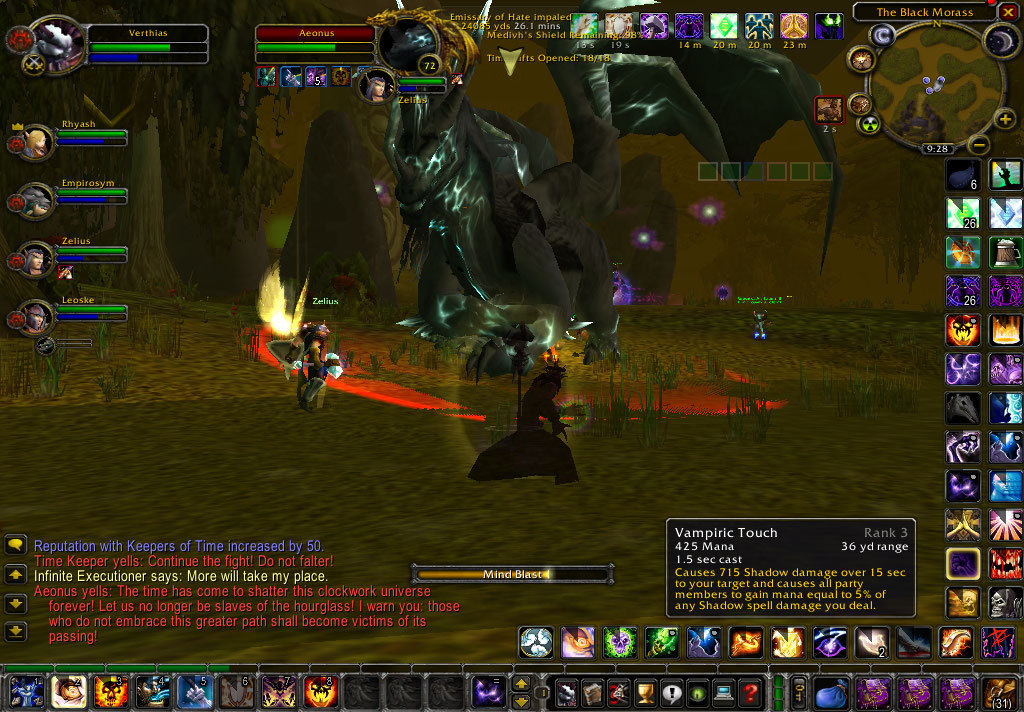
\includegraphics[height=10cm]{mainmatter/imgs/wow.jpg}
  \caption{Počítačová hra World of Warcraft}
  \label{fig:comenius}
\end{figure}


\subsection{Vyuzitie}
\paragraph{MMO hry}
Hlavný ciel tejto práce je vytvorenie nástoja na tvorbu MMO hier využívajúcich GPS. Avšak má i mnohé iné využitia. \
Dany framework moze byt taktiez vyuzity ako pomocka pre tvorbu edukativnych hier, či teambuildingových akcii. 

\paragraph{Turisticko-historicke prehliadky}
Ako príklad si môžeme uviesť: Turista si stiahne mobilnú aplikáciu pre android telefón, zapne GPS a pripoji sa na server. Hneď sa dozvie, že tam kde stojí práve teraz bol pred mnohymi rokmi chrám. Prečíta si informácie spolu s obrázkami. Poprípade keď sa poobzerá uvidi QR kód s logom Ďalší cieľ jeho cesty má už na mape vytýčený. A takto turista prejde trasu, ktorú pre neho pripravil sprievodca. 

\subsection{Technológie}


\paragraph{MVC} alebo model, view, controller architektura založená na rozdelení aplikácie do týchto troch zložiek. Model je tvorený dátami, ktoré reprezentuje v aplikácii a obsahuje tiež hlavnú logiku pre prácu s nimi. View sa stará o vizuálnu stránku, ktorá je ako výsledok prezentovaná používatelovi. Controller spracováva jednotlivé dopyty od používatela a stará sa o interakciu s modelom a view.
\begin{figure}[h]
  \centering
  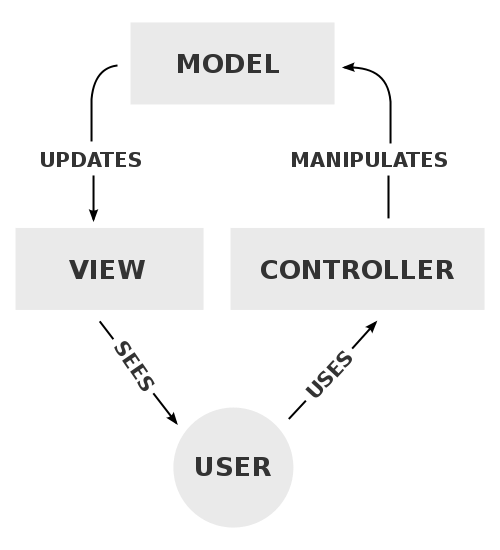
\includegraphics[height=10cm]{mainmatter/imgs/mvc.png}
  \caption{MVC architektúra}
  \label{fig:comenius}
\end{figure}


\paragraph{Android} Na strane klienta je zvolený operačný systém Android od firmy Google. Ktorý sa vačšinou používa práve na mobilných zariadeniach. Oproti konkurenčnému systému iOS od Apple je operačný systém open source. Ďalším argumentom bola politika schvalovania aplikácii a možnosť ich vyvýjať na rôznych operačných systémoch, kde pre android je to možné takmer pod každým operačným systémom. Ďaľšou možnosťou bol Windows Phone, ten však bol zavrhnutý kvôli . \
Android ma jadro založené na linuxe. Aplikácie možno vývíjať v jazyku Java pomocou Android SDK, ktorý ponúka funkcie na ovládanie zariadenia.


\paragraph{Bluetooth} je radiový štandard IEEE 802.15.1, ktorý slúži tiež na bezdotykovú komunikáciu medzi zariadeniami. Bol vytvorený firmou Ericsson v roku 1994. Pomenovaný je podľa dánskeho kráľa s menom Harald Blatand (do angličtiny prelozené ako Bluetooth), ktorému sa podarilo vďaka jeho diplomatickým schopnostiam uzmieriť kmene, ktoré proti sebe bojovali. Podla typu bluetooth vysielačov/prijímačov môžu mať navzajom dosah až po 400metrov. Najčastejšie sú však zariadenia s dosahom 10metrov. S novšími verziami bluetooth je možná rýchlosť prenosu dát až 24 Mbit za sekundu. Často sa používa na jednoduche posielanie dát medzi mobilnými zariadeniami či bezdrotovych slúchadlách. 


\paragraph{QR Kody} QR (Quick Response) sú čiarové kódy, v ktorých je uložená informácia. Boli vyvinuté japonskou automobilkou Toyota na rýchle čítanie informácii o tovare nimi označenými. Sú zložené z bielych a čiernych štvorcov usporiadaných v mriežke. Môžu byť vytlačené na papier a prečítané pomocou čítačiek či zariadení, ktoré zosnímajú kód a dokážu ho preložiť spať do pôvodnej informácie.  QR kódy sú často pridávané do reklamných plagátov či videí ako odkazy na produkty výrobcu. Nájdeme ich ale i pri kultúrnych pamiatkach ako ďaľší zdroj informacií. Využitia sú rôzne kedže na relatívne malej ploche dokážu uložit 7089 numerických, 4296 alfanumerických, 2953 binárnych či 1817 kanji znakov. QR kódy obsahujú tiež pripravenú opravu chýb pri mierne poškodenom QR kóde a tak je čítačka schopná prečítať informáciu napríklad, keď je kúsok QR kódu prekrytý. 

\begin{figure}[h]
  \centering
  
\includegraphics[height=10cm]{mainmatter/imgs/qr.png}
  \caption{QR kód}
  \label{fig:comenius}
\end{figure}

\paragraph{NFC} Možno ani netušite, že ste sa už s NFC stretli. Napríklad ak ste platili pri nákupoch pomocou karty bezdotykovo. NFC (Near field communcation) je pomerne mladá technológia, pomocou ktorej môžu zariadenia medzi sebou komunikovať na krátku vzdialenosť (maximálne 20 centimetrov) bezdotykovo. Je potomkom RFID - Rádiofrekvenčných identifikačných kariet a ich čítačiek, ktoré sa spojili v NFC. Takže dokáže komunikovať s obomi i ostatnými zariadeniami, ktoré NFC majú.


\subsection{Frameworky, knižnice a API}


\paragraph{jQuery} Je javascriptová knižnica, ktorá uľahčuje prácu hlavne pri manipulovaní s objektami na stránke, pri tvorbe efektov a to všetko pri zachovávaní kompatibility medzi rôznymi internetovými prehliadačmi.

\paragraph{Bootstrap} Je front-endovy hlavne framework pre tvorbu webových stránok. Poslúži nám na vytvorenie moderneho a funkčného designu  medzi webovými prehliadačmi. 

\paragraph{Codeigniter} open sourceovy PHP framework. Zakladá si na MVC architektúre avšak necháva volnosť programátorovi. Taktiež ako ďaľšiu z klúčových vlastností pre jeho výber bola jeho rýchlost. Na zahodenie nie sú ani knižnice a nástroje, ktoré ulahčujú vývoj aplikacie.

\paragraph{Google maps} Služba od internetového giganta Google pomocou, ktorej zobrazíme mapu réalneho sveta ale i toho fiktívneho, herného. Funguje ako javscriptová, css, html služba, ktorá má vśak svoje obmedzenie pri používaní zadarmo - 25 000 načítaní za deň.

\paragraph{Google directions} Ďalšia zo služieb, ktorú Google ponúka. Táto sa stará o navigáciu z bodu A do bodu B a poskytuje potrebné informácie pre potrebné pokyny.

\paragraph{QR code generator} Je na strane serveru jasnou volbou pre množstvo funkcii a parametrov, ktoré poskytuje pri tvorbe QR kodov. QR kody budú môcť byť generované užívateľmi a pridané do hry a tak prispievať a vyvíjat obsah do hry.
\href{http://phpqrcode.sourceforge.net/examples/index.php?example=006}{PHP QR code generator} 

\paragraph{ZBar} GPL knižnica pre Androidy pomocou, ktorej môžeme skenovať QR kódy. Vybraná je táto napriek obľúbenej knižnici zxing, ktorá pre svoje použitie sa musí stiahnuť ich aplikácia ktorej sa posiela požiadavok, čo by nebolo veľmi príjemné. ZBar sa teda bude zakomponovaný do našej klientskej android aplikácie.


\subsection{Podobné projekty}

\paragraph{Realm Crafter} Je komerčný nástroj na tvorbu MMORPG avšak na počítač. Dá sa pomocou neho relativne jednoducho vytvorit herný svet. Okrem ceny a trošku zložitejšej tvorby sveta sa dajú vytvoriť presvedčivé výsledky. Hlavným problémom je nemožnosť tvorby hier na smartphony využívajucích GPS.

\paragraph{Ingress} Je hra založená tiež na pohybe hráčov v reálnom svete a pomocou mobilných android zariadeni s GPS a internetovým pripojením pohybovaním v hernom svete. Hra je zadarmo a viac strategiou pre tímy. Avšak naším cielom je tvorba podobných hier a s prvkami RPG.

